\documentclass[letter,12pt]{article}
\usepackage{jheppub}
\usepackage{taro}
\usepackage{booktabs}

\usepackage{mathrsfs}
\usepackage{tcolorbox}
\newcommand{\red}[1]{\textcolor{red}{#1}}
\newcommand{\pink}[1]{\textcolor{pink}{#1}}
\newcommand{\blue}[1]{\textcolor{blue}{#1}}
\newcommand{\green}[1]{\textcolor{ForestGreen}{#1}}
\newcommand{\orange}[1]{\textcolor{orange}{#1}}
\newcommand{\brown}[1]{\textcolor{brown}{#1}}

\newcommand{\J}{\mathcal{J}}
\newcommand{\BO}{\mathcal{O}}
\newcommand{\OO}{\mathcal{O}}

\newcommand{\ab}[1]{\langle #1 \rangle}
\newcommand{\sqb}[1]{[ #1 ]}
\newcommand{\aMs}[3]{\langle #1|#2|#3]}  		% <1|2|3]
\newcommand{\aMMa}[3]{\langle #1|#2|#3\rangle}		% <1|Q_1.Q_2|3>
\newcommand{\sab}[1]{s_{#1}}
\newcommand{\twhite}[1]{\textcolor{white}{#1}}

\title{Quantum Error Correction in AdS/CFT}

\def\Tr{{\rm Tr}}
\def\MHVbar{${\overline{\rm MHV}}$}
\def\nn{\nonumber}
\def\NeqFour{${\cal N}=4$}
\def\Split{{\rm Split}}
\def\spa#1.#2{\left\langle#1\,#2\right\rangle}
\def\spb#1.#2{\left[#1\,#2\right]}
\def\sandmx#1.#2.#3{%
	\left\langle#1{\vphantom1}\right|{#2}\left|#3\right]}%
\def\delt#1{\delta^{(#1)}}
\def\eps{\epsilon}
\def\Ord{{\cal O}}
\def\tlambda{\tilde\lambda}
\def\draftnote#1{{\sl #1}}
\def\tp{\!+\!}
\def\sA{{\cal A}}
\def\Int#1{I^{(#1)}}

\author[a]{Taro V. Brown}

\affiliation[a]{Department of Physics, UC Davis, One Shields Avenue, Davis, CA 95616, USA }


% e-mail addresses: one for each author, in the same order as the authors
\emailAdd{tvbrown@ucdavis.edu}


\abstract{We review bulk reconstruction in	AdS/CFT and, in particular, how subregion dualities seemingly violate the time-slice axiom for quantum field theories. Treating the correspondence as a quantum error-correcting code (QECC) resolves these problems, and we give an in-depth description of a QECC toy model known as the 3-qutrit code. Finally, we provide a brief outlook on extensions of the models described.}
\begin{document} 
\maketitle
\flushbottom
\newpage
\section{Introduction}
The AdS/CFT correspondence is a duality relating a
$(d+1)$-dimensional bulk theory of gravity or string theory in anti-de Sitter (AdS) spacetime to a $d$-dimensional boundary conformal field theory (CFT). The correspondence provides a dictionary between the CFT and gravity sides. This project focuses on how one relates operators on the boundary to operators in the bulk. This might seem strange at first since the operators on the boundary live in one spacetime dimension lower than the bulks fields, and so one might expect the dictionary only to work in one direction, but as we will show, we are able to \textit{reconstruct} information in the bulk from data on the boundary. Further, one can reconstruct operators using only part of the boundary information. Here we will focus on Rindler reconstruction, as well as general subregion dualities using the causal wedge. 

Using this reconstruction, some subtleties and puzzles in the prescription appear. We will describe the problems and then show how treating AdS/CFT as a Quantum Error Correcting Code (QECC) resolves the problems. For this purpose, we introduce a toy model: the 3-qutrit model. The model is very coarse-grained, and we give a brief introduction on how to introduce more degrees of freedom by using tensor networks. The project is based mainly on the excellent review \cite{bib1}, while we also want to acknowledge the original papers \cite{bib2,bib3,bib4}. 
\section{Bulk Reconstruction \label{sec:1}}
We are going to consider global AdS spacetime with metric
\begin{equation}
	\begin{aligned}
		\dd s^2=&-\left(1-r^2\right)\dd t^2+\left(1-r^2\right)^{-1}\dd r^2+r^2\,\dd\Omega_{d-1}^2
		\\
		=&\omega(\rho)^2\left(-\dd t^2+\dd \rho^2+\sin^2\rho\,\dd\Omega_{d-1}^2 \right),
	\end{aligned}
\end{equation}
where we work in natural units, such that the AdS length $\ell_{\text{AdS}}\equiv 1$ and we have defined $r\equiv \tan\rho $ as well as the conformal factor $\omega(\rho)\equiv \frac{1}{\cos\rho}$ in the second line. This metric is conformally related to the Einstein Static Universe, and it's conformal structure can be illustrated on a cylinder. The boundary is located at $r=\infty$ and can be viewed as a cylindrical shell.

We are going to denote bulk coordinates by $x\equiv (r,t,\Omega)$ and boundary coordinates by $X\equiv (t,\Omega)$. The AdS/CFT duality provides a map between operators on the boundary $\OO(X)$ and operators in the bulk $\phi(x)$. This is illustrated using the global AdS cylinder on Figure \ref{fig:adscftfig1}.
\begin{figure}[]
	\centering
	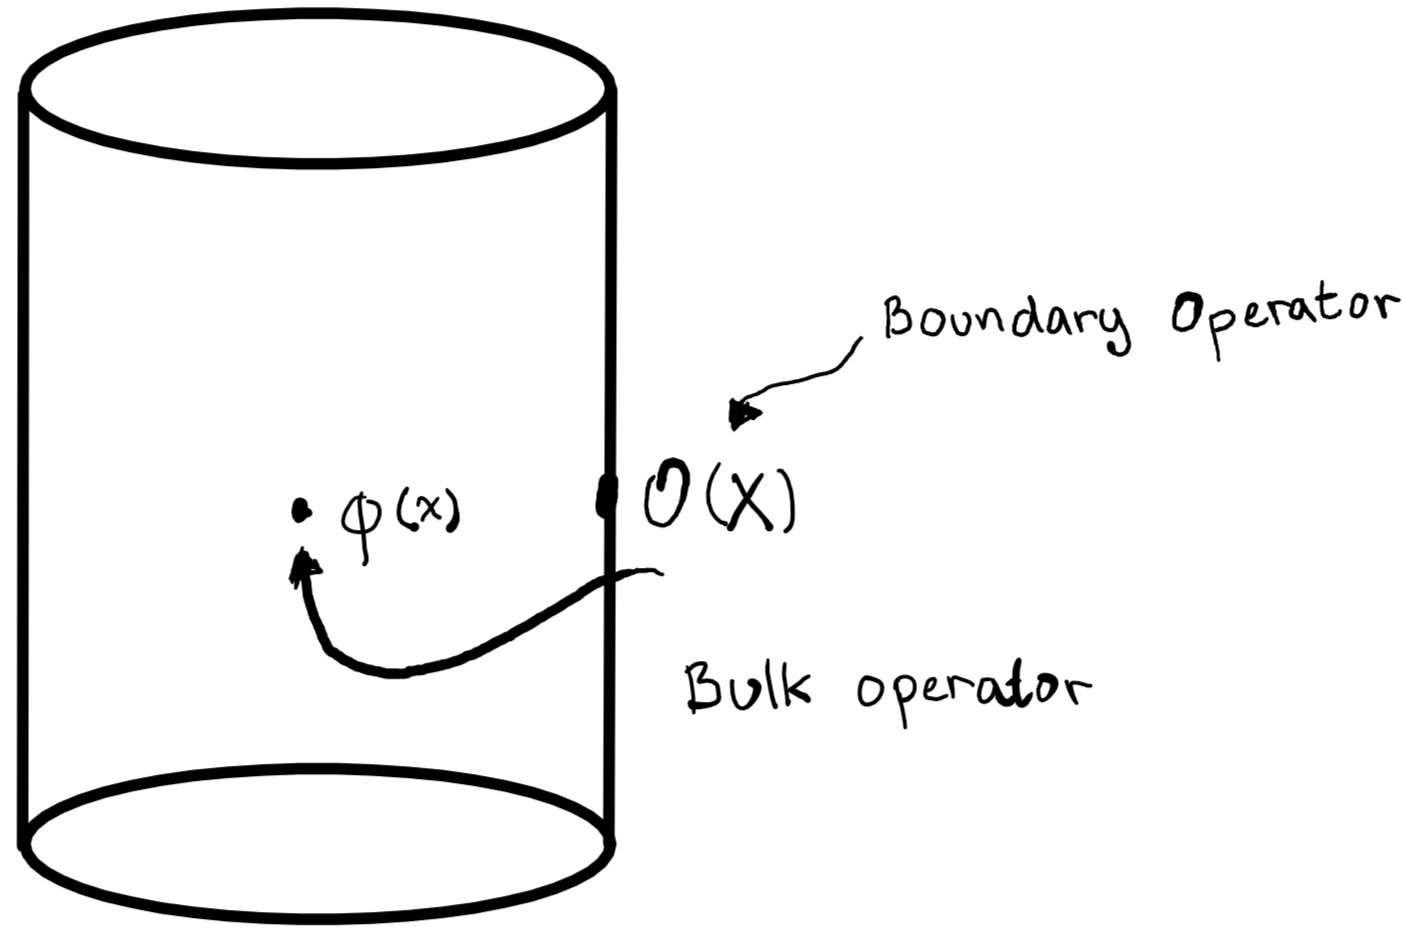
\includegraphics[width=0.6\linewidth]{ADS_CFT_Fig1}
	\caption{Global AdS as a cylinder with bulk operator $\phi(x)$ and boundary operator $\OO(X)$}
	\label{fig:adscftfig1}
\end{figure}
If one solves the equations of motion of the bulk field $\phi(x)$ near the boundary and demands that the solution is normalizable, the following extrapolate dictionary relates it to the boundary operator,
\begin{equation}
	\begin{aligned}
		\lim_{r\to \infty}r^{\Delta}\phi(x)=\BO(X)	\end{aligned}, \label{eq:1}
\end{equation}
where for a generic scalar of mass $m$, $\Delta$ satisfies $\Delta(\Delta-d)=m^2$. Going from the bulk to the boundary seems very natural and one can ask whether it is possible to obtain the full bulk solutions if the boundary operator is known. I.e. we are interested in solving the equations of motion of $\phi(x)$ under the boundary condition \eqref{eq:1}. 
As is often the case, the solution is a Greens function $ K(x;X)$ relating the boundary and the bulk as follows
\begin{equation}
	\begin{aligned}
		\phi(x)=\int\dd X K(x;X)\BO(X) \label{eq:2}
	\end{aligned}
\end{equation}
$ K(x;X)$ is often referred to as the \textit{smearing function}. If one takes a bulk point $x$, then $K(x;X)$ has support on set of boundary points that are spacelike separated from $x$, see Figure \ref{fig:adscftfig2}a. 

We are going to focus on constructing operators from boundary subregions. One such subregion is the Rindler wedge, $W$, defined by metric
\begin{equation}
	\begin{aligned}
		\dd s^2=-(\rho^2-1)\dd \tau^2+(\rho^2-1)^{-1}\dd \rho^2+\rho^2\dd H_{d-1}^2
	\end{aligned}
\end{equation}
with $\dd H^2_{d-1}=\dd \chi^2+\sinh^2\chi\dd \Omega_{d-2}^2$ being the metric on a $(d-1)$-dimensional hyperbolic ball. The metric has $\rho>1$ and $-\infty <\tau < \infty$ and its embedding in the global AdS cylinder is shown on Figure \ref{fig:adscftfig2}b. Using similar arguments to the global reconstruction, it can be shown explicitly that a bulk field can be reconstructed from a boundary operator if it lies within the Rindler wedge,
\begin{equation}
	\begin{aligned}
		\phi(x)|_{x\in W}=\int_{\partial W}\dd X K(x;X)\BO(X)
	\end{aligned}
\end{equation}
where $K(x;X)$ now only has support on the boundary region of the wedge. Using this as our starting point, we can find a version of \eqref{eq:2} for any subregion, using the causal wedge, $W_C$, for any boundary spatial subregion $A$ , defined by 
\begin{equation}
	\begin{aligned}
		W_C[A]=\mathscr{I}^+[D_\partial[A]]\cap\mathscr{I}^-[D_\partial[A]]
	\end{aligned}
\end{equation}
The bulk field can the be reconstructed on the boundary region $A$ as long as it is in the causal wedge, see Figure \ref{fig:adscftfig2}c. 
\begin{figure}[]
	\centering
	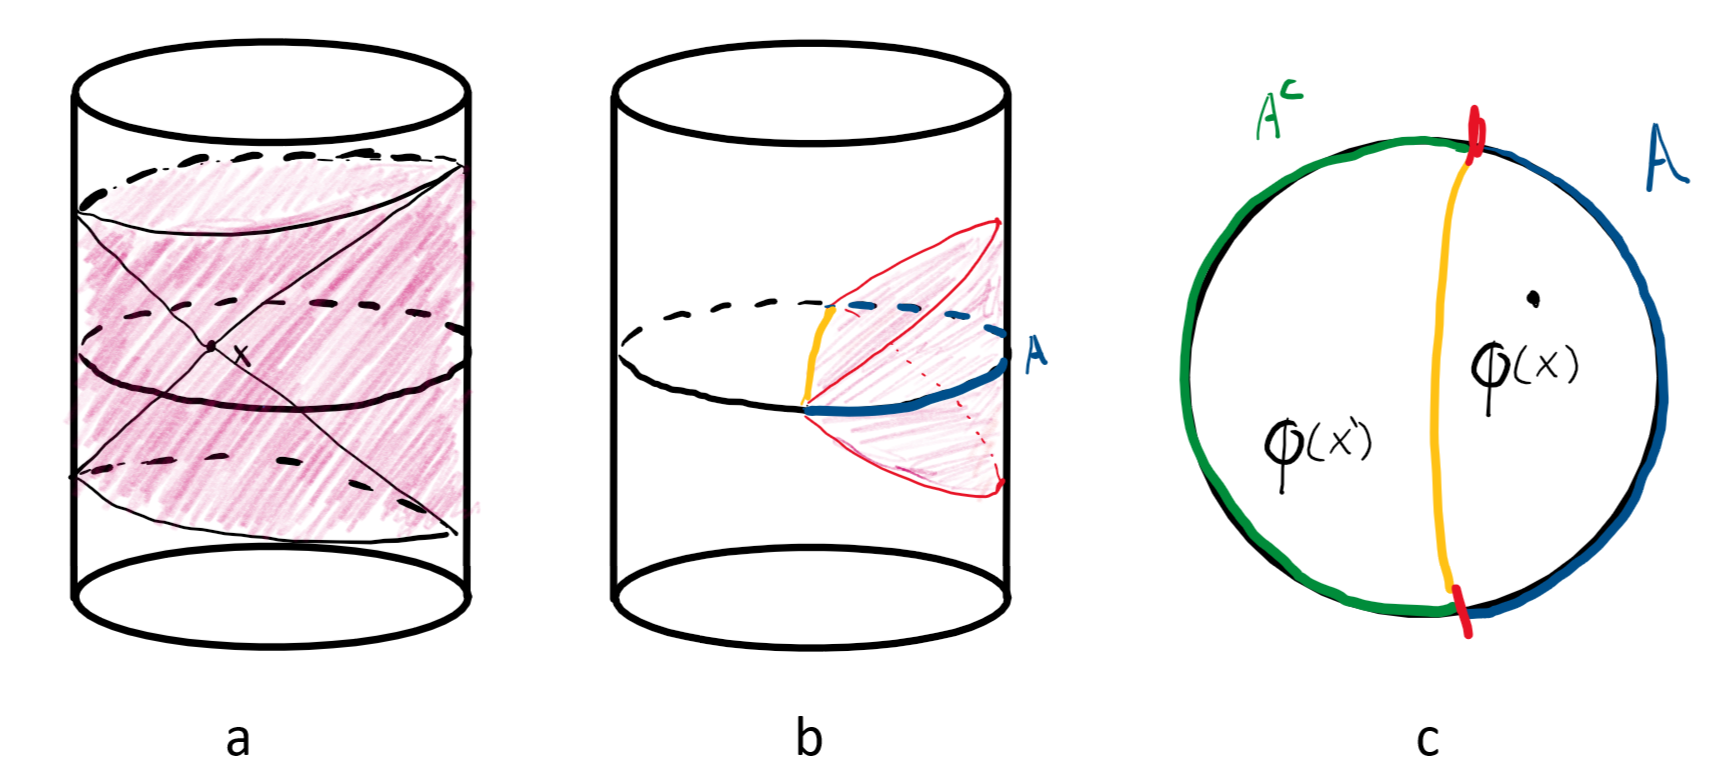
\includegraphics[width=0.95\linewidth]{ADS_CFT_Fig2}
	\caption{a) Global reconstruction of bulk point $x$. The smearing function has support on the set of boundary points that are spacelike separated from $x$ which is illustrated in purple on the plot. b) Rindler wedge in global Ads cylinder. c) Constant time-slice  of a general subregion-reconstruction. $\phi(x)$ has support on region $A$, while $\phi(x')$ does not.}
	\label{fig:adscftfig2}
\end{figure}
Using these definitions we arrive at two puzzles, which we will describe below.
\subsubsection*{Radial Commutivity Puzzle}
Using the reconstruction procedure just described on a $t=0$ timeslice with support on a region $A$ that covers almost the whole boundary region, as shown on the first part of Figure \ref{fig:adscftfig3}, one finds that the operator dual to $\phi$ on the boundary, will necessarily commute with an operator $\OO$ that lies in the complement region $A^C$. 
\begin{equation}
	\begin{aligned}
		\left[\phi(x),\BO(X')\right]=0
	\end{aligned}
\end{equation}
Similarly one can pick a different operator $\OO '$ on the boundary and by using a new region $A'$, see Figure \ref{fig:adscftfig3}b, we once again find that $\phi$ commutes with $\OO '$. We can in fact do this with all operators and so must conclude that $\phi$ commutes with \textit{all} operators on the boundary.
\begin{figure}[]
	\centering
	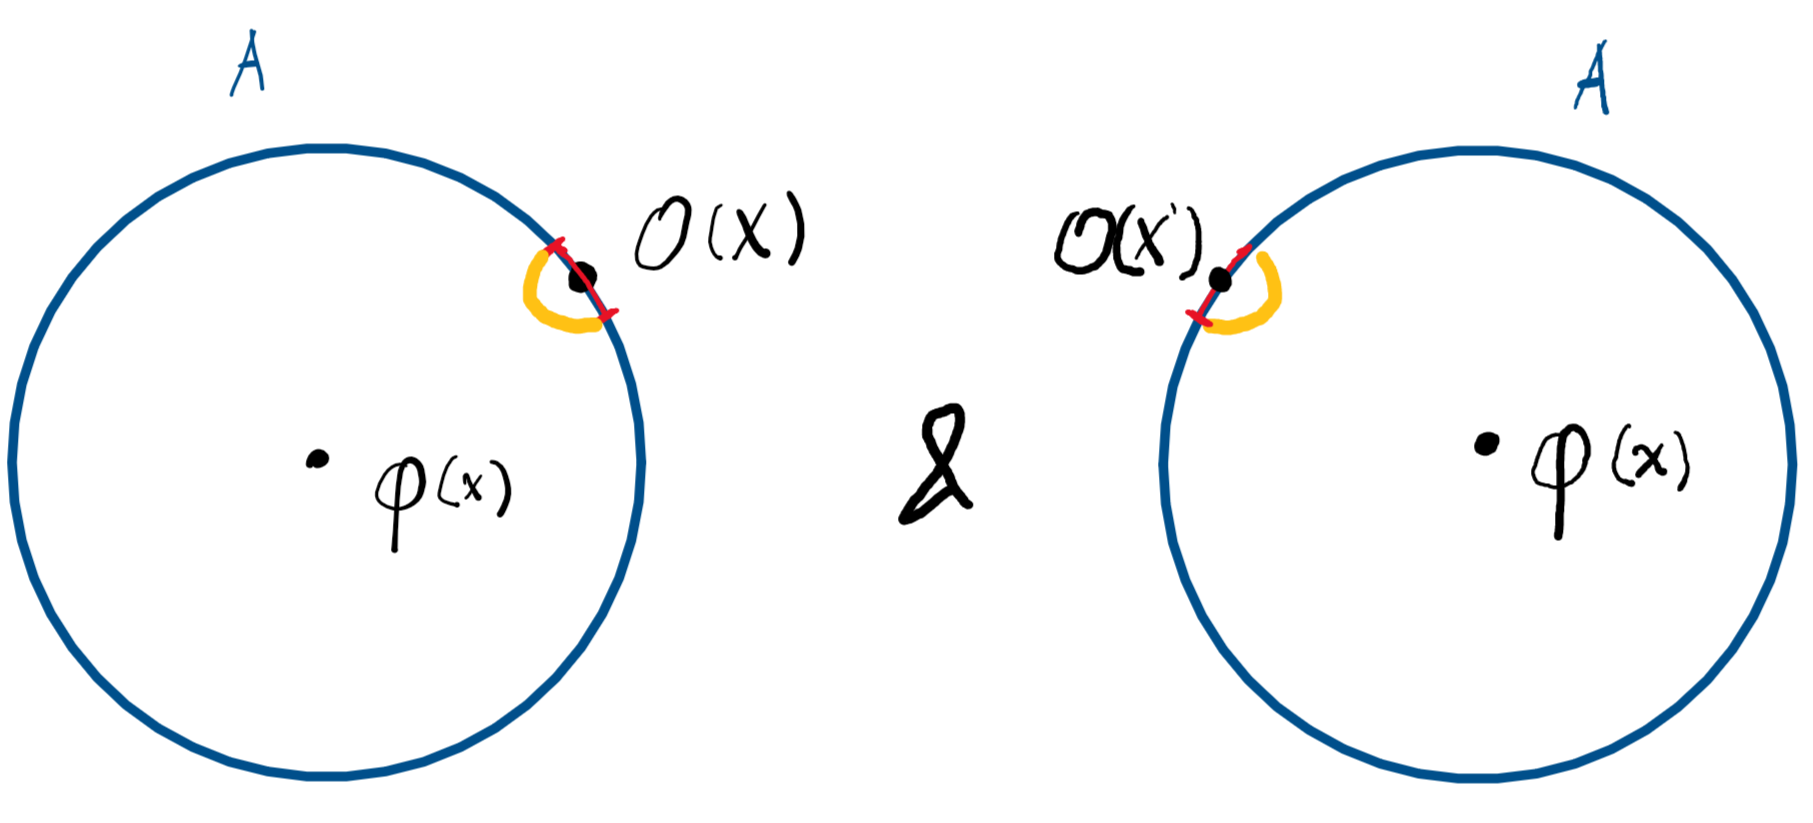
\includegraphics[width=0.75\linewidth]{ADS_CFT_Fig3}
	\caption{Both figures display a constant time-slice. On the first figure $\phi(x)$ can be reconstructed on the boundary to commute with $\OO(X)$ using the subregion duality. Similarly, the second figure shows how one can reconstruct $\phi(x)$ on the boundary to commute with another operator $\OO(X')$. This procedure holds for all operators and so $\phi(x)$ commutes with all operators on the boundary.}
	\label{fig:adscftfig3}
\end{figure}
This however contradicts a well-known quantum field theory theorem known as the \textit{time-slice axiom}, which states that any operator which commutes with all local operators at a fixes time most be trivial. Since $\phi$ obviously is not trivial this is quite puzzling.

\subsubsection*{ABC Puzzle}
The ABC-puzzle is best illustrated through Figure \ref{fig:adscftfig4}. Using the reconstruction procedure $\phi$ can not be reconstructed on regions $A$, $B$, or $C$, it can however be reconstructed from any combination of two regions. So there exists at least 3 representation of $\phi$: $\phi_{AB},\; \phi_{BC},$ and $\phi_{CA}$. The can not be the same operator on the CFT however, and so we get yet another puzzle. 
\begin{figure}[]
	\centering
	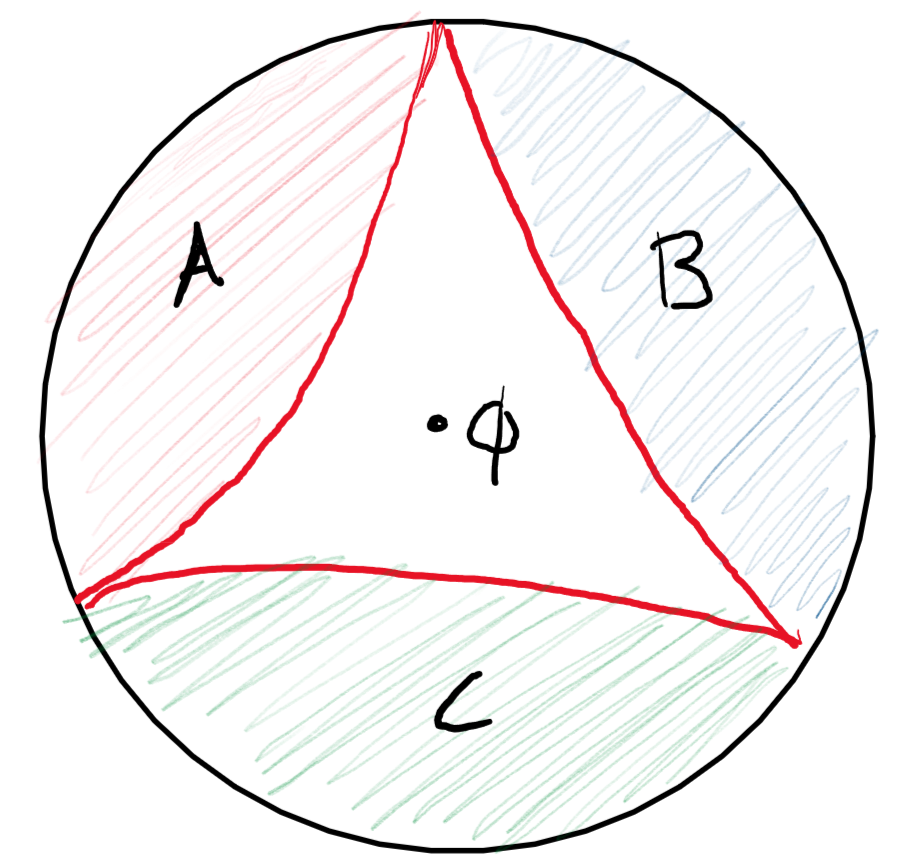
\includegraphics[width=0.3\linewidth]{ADS_CFT_Fig4}
	\caption{Constant time-slice. $\phi$ can be reconstructed on any
combination of two regions, i.e. $AB$, $BC$, $CA$.
}
	\label{fig:adscftfig4}
\end{figure}

Both puzzles can however be resolved by interpreting the correspondence as an quantum error correcting code, which we will describe next.

\section{Quantum Error Correction - The Qutrit Model}
Error correction is the procedure off protecting information from being lost. The type of loss depends on the situation, but if one is talking about quantum information it could e.g. be decoherence. 

In classical computers an easy way to protect information is through redundancy - simply sending your information multiple times. In quantum mechanics however, we are not able to procure our quantum bits (or, as we will see below, qutrits) in the same state due to the no-cloning theorem. Instead we have to come up with a new way to protect information. 

For this purpose we are going to define the 3-qutrit model. The qutrit is a 3 dimensional extension of the qubit (i.e. Bell state) and it has basis $\{\ket{0},\ket{1},\ket{2}\}$. Using these, Alice wants to send a qutrit $\ket{\psi}$ to Bob
\begin{equation}
	\begin{aligned}
		\ket{\psi}=\sum_{k=0}^{2}c_k \ket{k}
	\end{aligned}
\end{equation}
We will refer to this as the \textit{logical qutrit}. She wants to do it in a way that preserves the original qutrit even if part of the information is lost. To do this she encodes the information in terms of a 3-qutrit state:
\begin{equation}
	\begin{aligned}
		|\tilde \psi\rangle=\sum_{k=0}^{2}c_k \tilde{\ket{k}}
	\end{aligned}
\end{equation}
where the basis vectors now are
	\begin{equation} \label{eq:masslessSH}
		\begin{aligned}
			|\tilde 0\rangle &=\frac{1}{\sqrt{3}}\left(\ket{000}+\ket{111}+\ket{222}\right)\\
			|\tilde 1\rangle &=\frac{1}{\sqrt{3}}\left(\ket{012}+\ket{120}+\ket{201}\right)\\
			|\tilde 2\rangle &=\frac{1}{\sqrt{3}}\left(\ket{021}+\ket{102}+\ket{210}\right)\\
		\end{aligned}
	\end{equation}
such that $\left\{|\tilde k\rangle\right\}$ forms a basis for a 3-dimensional subspace, denoted by $H_{\text{code}}$, within the full 27 dimensional Hilbert space. The 3 qutrits encoding the information of the logical qutrit are called \textit{physical qutrits}. 

Before we move on, let us summarize some important features of the states just defined:
\begin{itemize}
	\item $H_{\text{code}}$ is symmetric under exhange of the 3 qutrits.
	\item All $| \tilde \psi \rangle\in H_{\text{code}}$ are highly entangled, since the density matrix obtained from tracing out two qutrits, i.e.
	\begin{equation}
		\begin{aligned}
			\rho_{\text{single qutrit}}=\frac{1}{\sqrt{3}}
			\left(\dyad{0}{0}+\dyad{1}{1}+\dyad{2}{2}\right)	\end{aligned}
	\end{equation}
is a maximally mixed state. 
\item Any single qutrit has no information about the original state.
\item Any two of the three qutrits contains complete information about the original state, so even if Bob looses a single qutrit he can still recover the original information. We will describe how this works below.
\end{itemize}
To see that the physical qutrits contain all the information from the logical qutrit, we define decoding operators $U_{ij}$, for $\{i,j\}=1,2,3$, $i\neq j$. It is easiest to see how these work through an explicit example, so take e.g. $U_{12}$, which has the explicit action of changing the first two qutrits in the following manor,
\begin{align}
	\begin{tabular}{ l c r }
		$|00\rangle\to|00\rangle$ & $|11\rangle \to |01\rangle$ & $|22\rangle\to |02\rangle$ \\ 
		$|01\rangle \to |12\rangle$ & $|12\rangle \to |10\rangle$ & $|20\rangle \to |11\rangle$ \\
		$|02\rangle\to |21\rangle$ & $|10\rangle\to|22\rangle$ & $|21\rangle \to |20\rangle$ 
	\end{tabular}.
\end{align}
Such that, for instance acting on the $|\tilde 1\rangle$ state
\begin{equation}
	\begin{aligned}
		U_{12}|\tilde 1\rangle&=\frac{1}{\sqrt{3}}\left(\ket{122}+\ket{100}+\ket{111}\right)
		\\
		&=\ket{1}_1\otimes \ket{\chi}_{23}
	\end{aligned}
\end{equation}
where $\ket{\chi}_{23}$ is the following state of the last two qutrits
\begin{equation}
	\begin{aligned}
		\ket{\chi}_{23}&\equiv \frac{1}{\sqrt{3}}\left(\ket{00}+\ket{11}+\ket{22}\right)
	\end{aligned}
\end{equation}
in general one finds $	U_{12}|\tilde k\rangle=\ket{k}_1\otimes \ket{\chi}_{23}$, 
such that we can recover the original state using the decoder
\begin{equation}
	\begin{aligned}
		U_{12}|\tilde \psi\rangle
		&=\ket{\psi}_1\otimes \ket{\chi}_{23}.
	\end{aligned}
\end{equation}
Using this operator Bob would be able to get the information from the logical qutrit, even if he lost the third physical qutrit somehow.
One then obviously has similar actions for $U_{31}$ and $U_{23}$. Now let us assume that Bob want to perform a quantum computation on the logical qutrit, i.e. he wants to act on it with a general linear operator,
\begin{equation}
	\begin{aligned}
		O\ket{k}=O_{jk}\ket{j}.
	\end{aligned}
\end{equation}
If he receives the encoded state $|\tilde \psi\rangle$, he wants an operator that gives the same value as above, i.e.
\begin{equation}
	\begin{aligned} \label{eq:3}
		\tilde{O}|\tilde k\rangle =O_{jk}|\tilde j\rangle 
	\end{aligned}
\end{equation}
An example of such an operator can be build from the decoding operators that we just defined, e.g.
\begin{equation}
	\begin{aligned}
		\tilde{O}_{12}\equiv U^\dagger_{12}O_1 U_{12},
	\end{aligned}
\end{equation}
where $O_1$ is an operator acting on the first qutrit.
This exactly has the intended action, i.e. satisfies \eqref{eq:3}, and since it only acts on the $1,2$ subset, once again Bob could loose the third qutrit and still perform his computation. 

Further, we can define similar operators $\tilde{O}_{31},\tilde{O}_{23}$. They are all different operators in the full Hilbert space, but they act in the same way in the code subspace. We will now discuss how this resolves both the puzzles encountered in section \ref{sec:1}
\section{AdS/CFT as a QECC}
\subsubsection*{Solution to ABC-puzzle}
We have just seen how the 3-qutrit model has operators that act the same way in a subspace, but are different operators in the full Hilbert space. Using this we can resolve the ABC puzzle. The idea is to identity 
\begin{itemize}
	\item 3 physical qutrits $\sim$ local degrees of freedom in the CFT.
	\item Logical qutrit $\sim$ bulk operator.
	\item $\phi_{AB},\phi_{BC},\phi_{CA}\sim \tilde{O}_{12},\tilde{O}_{23},\tilde{O}_{31}$
\end{itemize}
This notion is exemplified in Figure \ref{fig:adscftfig5}.
\begin{figure}[H]
	\centering
	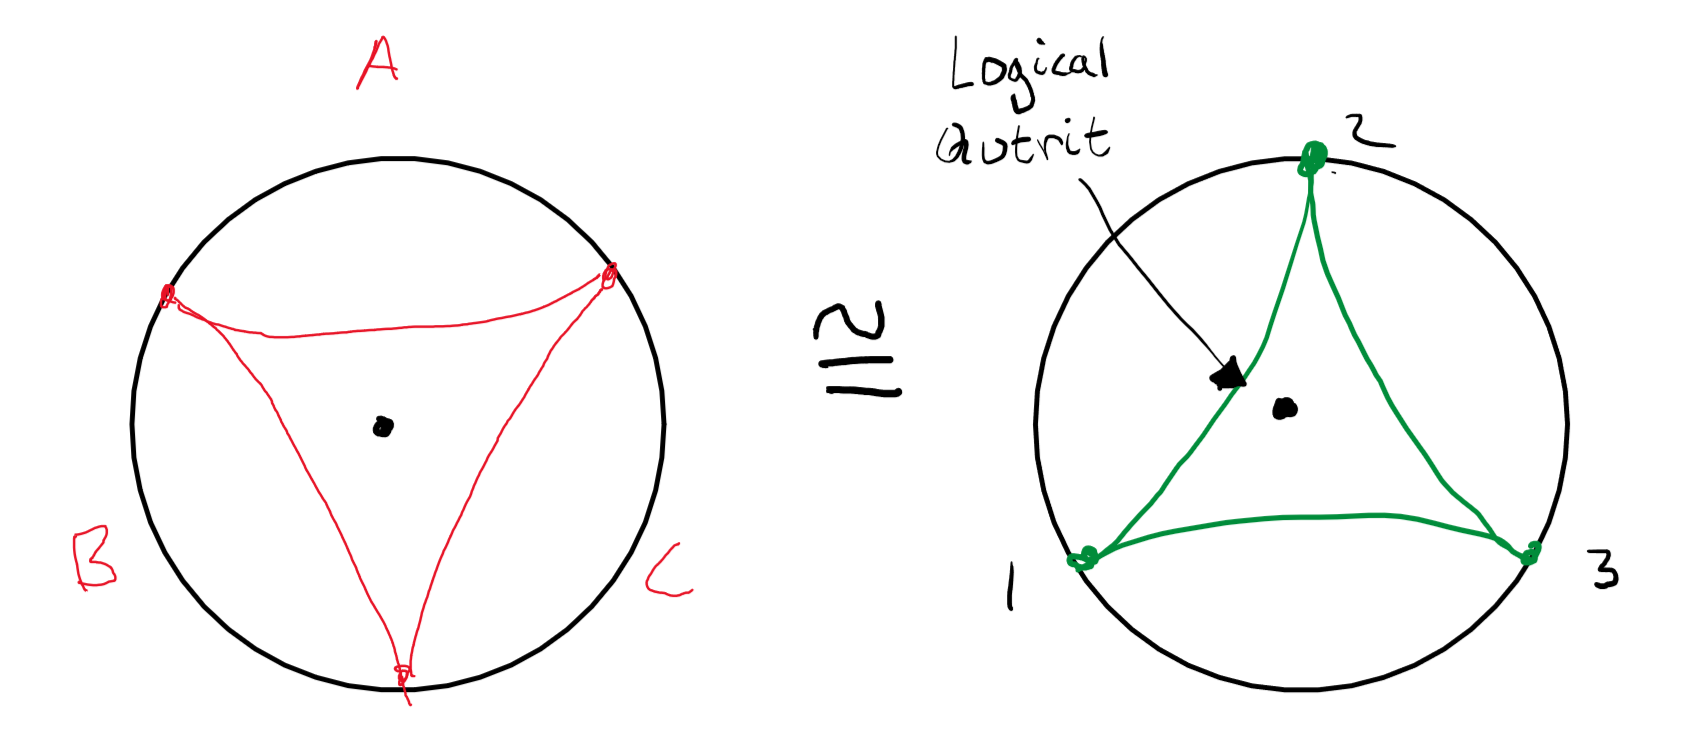
\includegraphics[width=0.85\linewidth]{ADS_CFT_Fig5}
	\caption{The ABC puzzle can be resolved by considering 3 local degrees of freedom of the CFT as the 3 physical qutrits.}
	\label{fig:adscftfig5}
\end{figure}
Further, in this setup equation \eqref{eq:2} only has support when states lie in $H_{\text{code}}$, where the code subspace are define das states that are perturbatively close to the vacuum.
\subsubsection*{Solution to Radial Commutivity Puzzle}
Thinking of AdS/CFT as a QECC also resolves the second puzzle, since the commutator can be zero and still be in agreement with the time-slice axiom if we take it in the code subspace as follows,
\begin{equation}
	\begin{aligned}
		\langle \tilde \psi_r |\left[\phi(x),\BO(X)\right]|\tilde \psi_l\rangle =0,~~~~~~~~\forall~~~~ |\tilde \psi\rangle\in H_{\text{code}}
	\end{aligned}
\end{equation}
In terms of the 3-qutrit model, we identify the bulk operators with $\tilde O$, and so we could write it as
\begin{equation}
	\begin{aligned}
		\langle \tilde \psi_r |[\tilde O,Y_i]|\tilde \psi_l\rangle =0,
	\end{aligned}
\end{equation}
where $Y_i$ is an operator acting on the $i$'th qutrit, and we can choose $\tilde O$ in every instance such that it acts on different qutrit pairs and so commutes with all local operators in our subspace.
\subsubsection*{Perspectives}
Having addressed the puzzles we are now left with a question - which states are not included in the code subspace? A good guess is a black hole, since states behind the horizon are not accessible by an asymptotic observer. Further, this is in line with the definition of states in the subspace as being asymptotically close to the vacuum, since if we keep increasing the energy of a a state it will naturally create a black hole. This is illustrated on Figure \ref{fig:adscftfig6}.
\begin{figure}[]
	\centering
	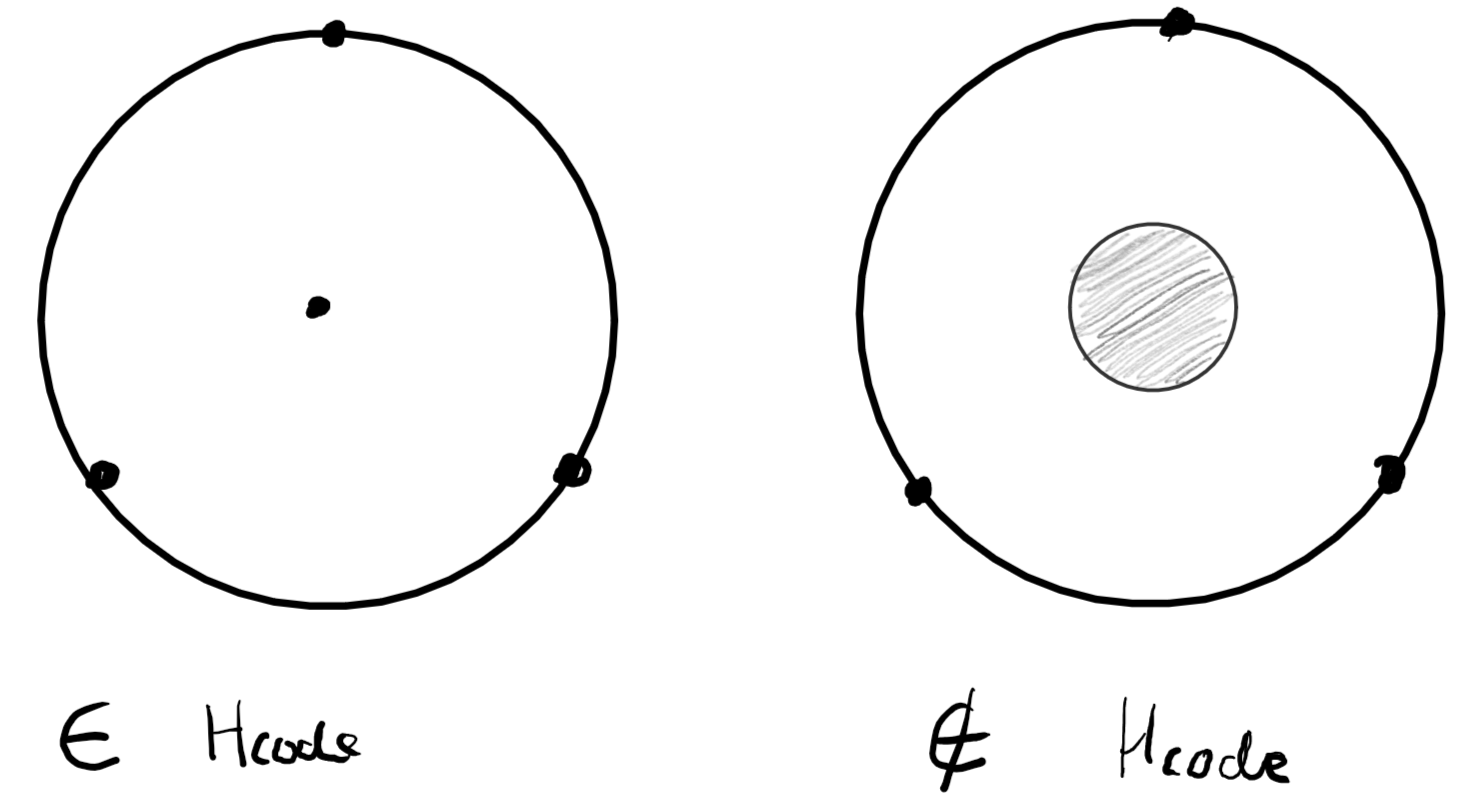
\includegraphics[width=0.7\linewidth]{ADS_CFT_Fig6}
	\caption{States not in the code subspace are states inside black holes.}
	\label{fig:adscftfig6}
\end{figure}

Further, we observe that the radial coordinate in this setup, describes how protected a state is to errors. A state placed in the center can for instance have multiple boundary regions erased but still be fine, while a state close to the boundary only needs a small region to be erased, for the state to have an error. This is shown in Figure \ref{fig:adscftfig7}.
\begin{figure}[]
	\centering
	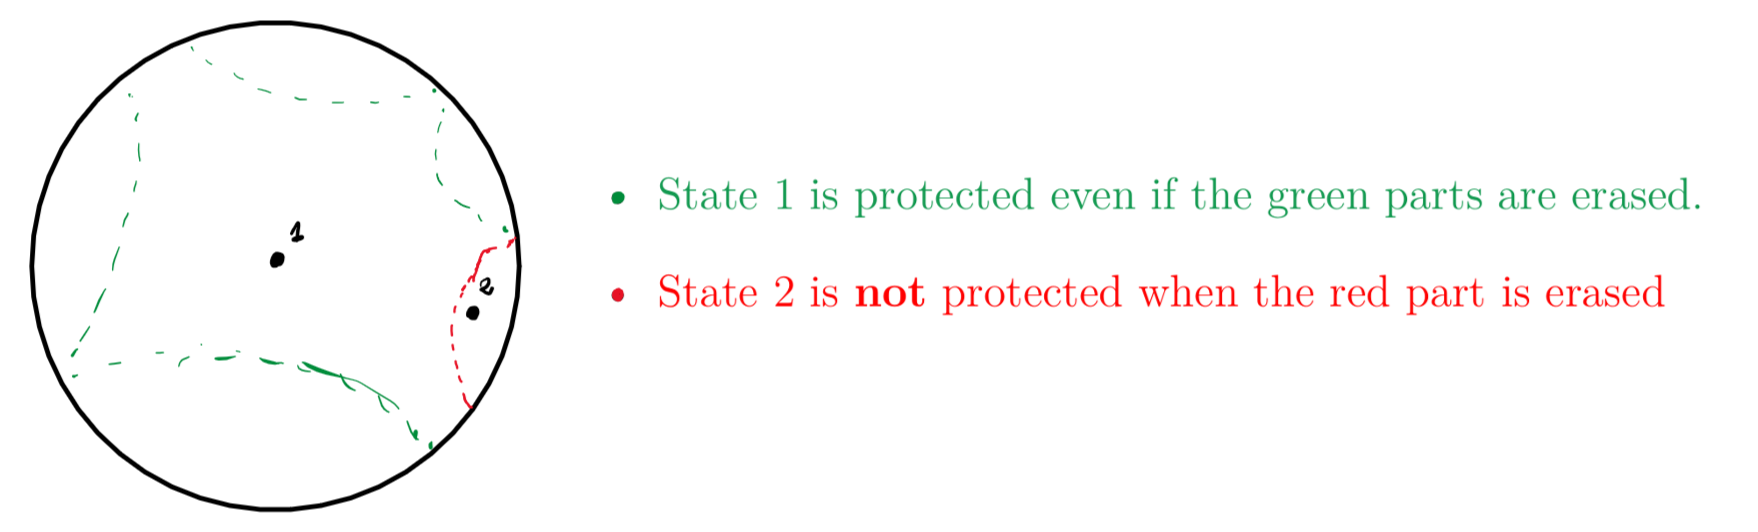
\includegraphics[width=0.9\linewidth]{ADS_CFT_Fig7}
	\caption{Protection level against erasure depends on the radial coordinate. The 1st qutrit has the largest level of protection.}
	\label{fig:adscftfig7}
\end{figure}

Finally the 3-qutrit model is very coarse-grained since it only allows for three degrees of freedom on the CFT. One way to get around this is by considering tensor models. In particular one can consider isometric tensors, that represent linear maps between Hilbert spaces 
\begin{equation}
	\begin{aligned}
		T: H_A\to H_B
	\end{aligned}
\end{equation}
Given a two-dimensional basis the map would e.g. be
\begin{equation}
	\begin{aligned}
		\ket{a}\to \sum_b T_{ab}\ket{b}
	\end{aligned}
\end{equation} 
Which can be illustrated graphically as\\ 
\begin{center}
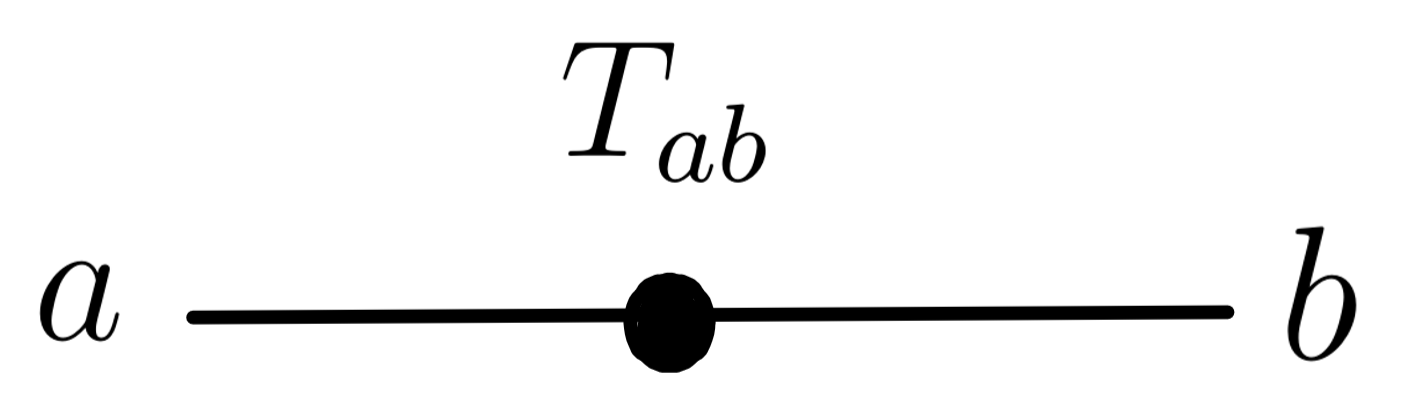
\includegraphics[width=0.25\linewidth]{ADS_CFT_Fig9}.
\end{center}

If one has tensors with a higher number of indices, there are simply more lines connecting the dot representing $T$. A tensor model of particular interest contains \textit{perfect tensors} which all have the same number of indices and obeys the property that any balanced bipartition $|A|=|A^C|$ of the indices
into inputs and outputs gives a unitary transformation $T$.

The three qutrit code is an example of such a model, which has 4 indices and a bond dimension (i.e. number of basis-elements) of $D=3$.
Another model of interest is the 6-index $D=2$ model. Both models are illustrated as tensors in Figure \ref{fig:adscftfig8}.
\begin{figure}[htb]
	\centering
	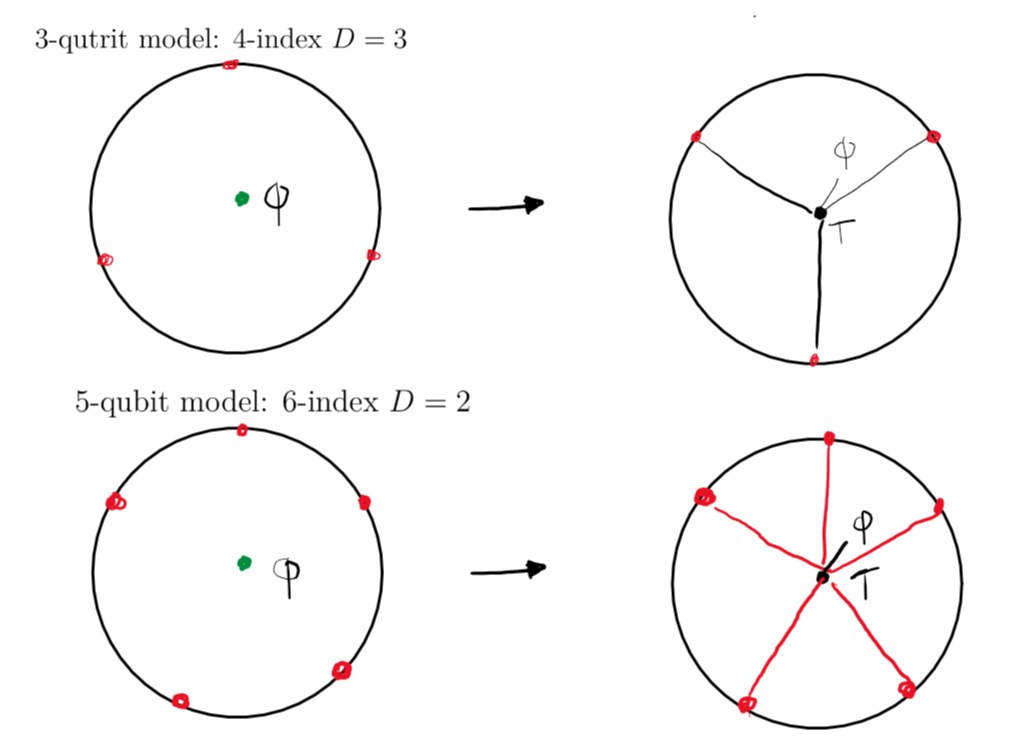
\includegraphics[width=0.95\linewidth]{ADS_CFT_Fig8}
	\caption{Depiction of how the 3-qutrit (top) and 5-qubit (bottom) models look as perfec tensor models. The tensor T has a free leg connecting to the logical qubit/qutrit.}
	\label{fig:adscftfig8}
\end{figure}

 Using the notion of tensors, one can create tensor networks. Using the 6-index perfect tensor model the authors of \cite{bib3}, created the HaPPY code, which is much less coarse-grained, compared to the toy-model described in this project. We have illustrated this tensor model with 3 levels in Figure \ref{fig:adscftfig10}. Other extensions such as the random tensor model exists. 
 
 There are many other features of the perfect tensor model that we have not discussed and we refer to \cite{bib1} for a more in-depth review.
 \begin{figure}[H]
 	\centering
 	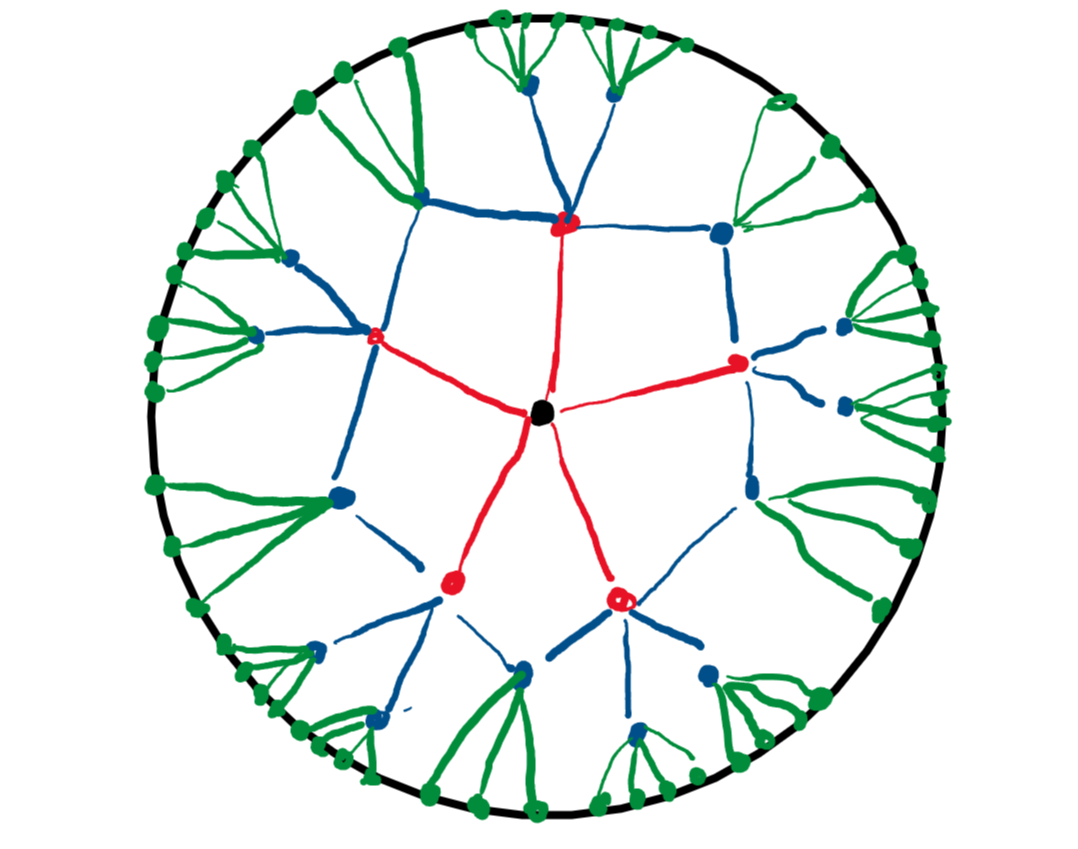
\includegraphics[width=0.35\linewidth]{ADS_CFT_Fig10}
 	\caption{A network of perfect 5-index $D=2$ tensors. Each level has its on color. By adding more levels, one can obtain models with more degrees of freedom both in the bulk and on the boundary.}
 	\label{fig:adscftfig10}
 \end{figure}
\section{Conclusion}
In the project we have reviewed how bulk operators can be reconstructed from boundary data in AdS/CFT. In this reconstruction several puzzles arise. We then introduced the notion of Quantum Error Correcting Codes and showed how thinking of the duality as a QECC resolved the puzzles.

Finally we briefly discussed extensions of the QECC toy model introduced using perfect tensor networks. 

The study of the gauge/gravity correspondence is a rich field with many applications outside of high energy theory, and understanding the duality better will hopefully propagate to a understanding various phenomenon in other areas of physics, as well as uncovering basic structures of our universe.
%%%%%%%%%%%%%%%%%%%%%%%%%%%%%%
%%%%%%%%%%%%%%%%%%%%%%%%%%%%%%
%%%%%%%%%%%%%%%%%%%%%%%%%%%%%%
%%%%%%%%%%%%%%%%%%%%%%%%%%%%%%
%%%%%%%%%%%%%%%%%%%%%%%%%%%%%%
%%%%%%%%%%%%%%%%%%%%%%%%%%%%%%
%%%%%%%%%%%%%%%%%%%%%%%%%%%%%%
%%%%%%%%%%%%%%%%%%%%%%%%%%%%%%
%%%%%%%%%%%%%%%%%%%%%%%%%%%%%%
\newpage
\begin{thebibliography}{99}
	%\cite{Harlow:2018fse}
	\bibitem{bib1}
	D.~Harlow,
	%``TASI Lectures on the Emergence of Bulk Physics in AdS/CFT,''
	PoS \textbf{TASI2017}, 002 (2018)
%	doi:10.22323/1.305.0002
	[arXiv:1802.01040 [hep-th]].
	%106 citations counted in INSPIRE as of 16 Mar 2022	
	%\cite{Almheiri:2014lwa}
	\bibitem{bib2}
	A.~Almheiri, X.~Dong and D.~Harlow,
	%``Bulk Locality and Quantum Error Correction in AdS/CFT,''
	JHEP \textbf{04}, 163 (2015)
%	doi:10.1007/JHEP04(2015)163
	[arXiv:1411.7041 [hep-th]].
	%480 citations counted in INSPIRE as of 16 Mar 2022
	%\cite{Pastawski:2015qua}
	\bibitem{bib3}
	F.~Pastawski, B.~Yoshida, D.~Harlow and J.~Preskill,
	%``Holographic quantum error-correcting codes: Toy models for the bulk/boundary correspondence,''
	JHEP \textbf{06}, 149 (2015)
%	doi:10.1007/JHEP06(2015)149
	[arXiv:1503.06237 [hep-th]].
	%508 citations counted in INSPIRE as of 16 Mar 2022
	%\cite{Dong:2016eik}
	\bibitem{bib4}
	X.~Dong, D.~Harlow and A.~C.~Wall,
	%``Reconstruction of Bulk Operators within the Entanglement Wedge in Gauge-Gravity Duality,''
	Phys. Rev. Lett. \textbf{117}, no.2, 021601 (2016)
	%doi:10.1103/PhysRevLett.117.021601
	[arXiv:1601.05416 [hep-th]].
	%343 citations counted in INSPIRE as of 16 Mar 2022
\end{thebibliography}
\end{document}

